\section{Text Analysis Queries and Demonstration}
Our demonstration will illustrate the following points: 
\begin{enumerate}
  \item The ability to perform statistical text analytics inside the DBMS
  \item Query driven computation of analytics
  \item The flexibility of our data sources by using structured data and text
  potentially across multiple domains
\end{enumerate} 
\subsection{Dataset for Example}
Our sample demonstration for MADden involves a variety of NFL based data sources. 
The data is represented in Table \ref{tab:madschema} as an abbreviated
schema\footnote{These tables may be extracted to an RDBMS, or defined over an
API using a foreign data wrapper (fdw).}.

The {\tt NFLCorpus} table holds semistructured data. Textual data from blogs,
news articles, and fan tweets, with document metadata such as timestamp, tags,
type, among others. The tweets were extracted using the Twitter Streaming API
with a series of NFL related keywords, and the news articles and blogs were
extracted from various sports media websites. These documents vary in size and
quality, with some potential out-of domain documents (mainly tweets).

The other tables are more structured,
including {\tt PlayerStats2011\_*}, with * indicating passing ({\tt Pass}), Receiving ({\tt
Rec}), Rushing ({\tt Rush}), Special Teams ({\tt ST}), or Defense ({\tt Def}).
This data was extracted from the NFL.com player database. Each table contains
the player's \textit{name}, \textit{position}, \textit{number}, and a series of
stats corresponding to the stat type (Some players show up in multiple tables, others in only one). The
{\tt Player} table holds information about a player in the NFL, including
\textit{college}, \textit{birthday}, \textit{height}, \textit{weight}, as well
as \textit{years\_in\_NFL}. The {\tt Team} table holds some basic information
about the 32 NFL teams, including \textit{location}, \textit{conference}, \textit{division}, and \textit{stadium}.
{\tt TeamStats\_2011} holds the team rankings and stats in a vareity of categories (Offense, Defense, Special Teams,
Points, etc.).
{\tt Extracted\_Entities} can either be a view or table, and it stores the
extracted entities found in the {\tt NFLCorpus} documents.

\begin{table}
\begin{center}
\begin{tabular}{|l|l|}
\hline
\multicolumn{2}{|c|}{Example Schema}\\
\hline
$NFLCorpus$ & \textit{doc\_id, type, text, tstmp, tags, \ldots}\\
\hline
$PlayerStats2011\_*$ & \textit{pid, specific stats\ldots }\\
\hline
$Player$ & \textit{pid, f\_name, l\_name, college, \ldots}\\
\hline
$Team\_Stats2011$ & \textit{team, points, pass\_yds, stats\ldots}\\
\hline
$Team$ & \textit{team, city, state, stadium, \ldots}\\
\hline
$Extracted\_Entities$ & \textit{doc\_id, entity, \ldots} \\
\hline

\end{tabular}
\end{center}
\caption{Abbreviated NFL dataset schema}
\label{tab:madschema}
\end{table}

\subsection{Text Analytics Queries}
Based on our example dataset, suppose a sports journalist
wants to do an investigative piece on overall public opinion 
of all Florida-based NFL teams during the 2011-2012 season. 
Such a peice would require in-depth analysis of news reports,
tweets, blog postings, among other sources. The standard approach would
consist of trawling through the text sources either by hand
with help, or using a series of different text processing
toolkits and packages, sometimes specialized for a singular 
task. Instead of multiple tools, MADden can streamline this process, with its
declarative, in-database approach to text analytics. A first step could 
conceivably consist of paring your corpora down to just
the documents related to the Florida football teams, namely
the Miami Dolphins, Jacksonville Jaguars, and Tampa Bay Buccaneers. 

%\lstset{breaklines=true}
%\lstset{tabsize=2}
%\lstset{basicstyle=\small}
%\begin{lstlisting}{language=SQL}
\begin{small}
\begin{alltt}
\textit{Q1: Entity Resolution}
SELECT DISTINCT doc_id
FROM extracted_entities
WHERE match('Jaguars', entity) > match\_thresh
   OR match('Dolphins', entity) > match\_thresh
   OR match('Buccaneers', entity) > match\_thresh;
\end{alltt}
\end{small}
%\end{lstlisting}

The $match$ function used in Query 1 is an Entity
Resolution UDF which calculates a $[0,1]$ bound inverse metric, where terms that
are close to our target will have a higher score than those that are less
similar. $Extracted\_Entities$ is a view constructed using $entity\_find$. 
This function detects entities using one of two accuracy settings
(high accuracy with lower recognition, or low accuracy with higher
recognition), on textual documents as they are added to the database 
(In this case, likely news articles and blogs). Table \ref{tab:madfunct} shows some of
the current text analysis functions implemented in MADden. \\

\begin{table}
\begin{center}
\begin{tabular}{|l|l|}
\hline
\multicolumn{2}{|c|}{Functions}\\
\hline
$match(target, against)$ & Entity Resolution\\
\hline
$sentiment(text)$ & Sentiment Analysis\\
\hline
$entity\_find(text, boolean)$ & Detects Named Entities\\
\hline
$pos\_tag(text)$ & POS tagging\\
\hline
$viterbi$ & Part of speech tags using CRF  \\
\hline
$pos\_extract(text, type)$ & POS term extraction \\
\hline
\end{tabular}
\end{center}
\caption{Listing of current MADden functions}
\label{tab:madfunct}
\end{table}

Maybe the journalist wants to explore fan sentiment for the Jacksonville Jaguars
based on tweets collected during the NFL season. Utilizing the first 
query as a building block (with some changes), we can construct this 
query as follows:

%\lstset{breaklines=true}
%\lstset{tabsize=2}
%\lstset{basicstyle=\small}
%\begin{lstlisting}{language=SQL}
\begin{small}
\begin{alltt}
\textit{Q2: Entity Resolution and Sentiment Analysis}
SELECT DISTINCT E.docid, E.entity, sentiment(S.document)
FROM extracted_entities as E, NFLCorpus as S
WHERE E.doc_id = S.doc_id
  AND sentiment(S.document) in ('+', '-')
  AND match('Jaguars', E.entity) > match\_thresh
  AND S.type = 'tweet';
\end{alltt}
\end{small}
%\end{lstlisting}

In Query 2, one could accomodate for nicknames through OR-matching
the extracted entities, an alias table, among other strategies. Notice
that going from a singular text analytics task, to a more 
complex analysis only required a small change. Whereas a traditional
approach would have us either looking for a customized solution or patching
together packages, the declarative sql approach allows the user to just 
state what the result is.

And since we are working in SQL, we can combine queries on corpus 
tables with tables of structured data. For example, if our journalist
wants to analyze the media opinion of the state's best reciever,
he could consult both the player stats table, as well as the media blogs:

%\lstset{breaklines=true}
%\lstset{tabsize=2}
%\lstset{basicstyle=\small}
%\begin{lstlisting}{language=SQL}
\begin{small}
\begin{alltt}
\textit{Q3: Structured & Unstructured}
SELECT BestWR.name, sentiment(A.txt), A.txt
FROM NFLCorpus A, extracted_entities E,
         (SELECT P.fname || ' ' || P.lname as name
          FROM Player P, PlayerStats2011_Rec S
          WHERE S.pid = P.pid
            AND (   P.team = 'Jaguars' 
                 OR P.team = 'Dolphins' 
                 OR P.team = 'Buccaneers')
          ORDER BY S.rec_yds DESC
          LIMIT 1) as BestWR
WHERE E.doc_id = A.doc_id 
  AND (A.type = 'blog' OR A.type = 'news')
  AND match(BestWR.name, E.entity) > match\_thresh;
\end{alltt}
\end{small}
%\end{lstlisting}

Query 3, our final example, utilizes standard structured sql tables {\tt Player}
and {\tt PlayerStats2011\_Rec}, which represents players and their receiving
stats. Our journalist finds the best receiver playing on a Florida NFL team
based on receiving yards\footnote{Total yards over a season, yds/catch, and
touchdowns usually decides who the best receiver was at the end of a season.}.
Then, discover all the associated news and blog documents and perform entitiy
resolution function on the extracted entities, returning the sentiment and text
associated with that player. This method is not restricted to single domain
analytics. One can run analytics combining different datasets (e.g. State
Economies and the NFL), utilizing the same declarative in-database methods seen
here.

\subsection{User Interface}

During the conference, we plan to give an interactive demonstration of the 
{\system}'s capabilities. The demonstration will be based around MADden UI,
a web interface that allows users to perform analytic tasks on our dataset.
MADden UI has two forms of interaction: raw SQL queries, and a Mad
Lib\footnote{http://en.wikipedia.org/wiki/Mad\_Libs} style interface, with
fill-in-the-blank query templates for quick interaction as seen in Figure
2.

\begin{figure}
\begin{center}
	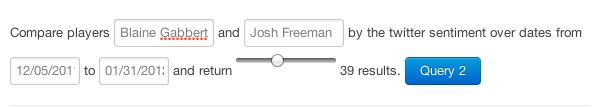
\includegraphics[scale=.43]{content/graphics/example_madlib.png}
\end{center}
\caption{Example MADden UI query template} 
\label{fig:madlib}
\end{figure}

For the demonstration, for ease of interpreting results, a series of
visualizations will be made available in the MADden UI. We will also provide
different datasets to combine and query upon using MADden as well.
